\section{Stabilisation de la dynamique par contrôle LQ}

%%%%%%%%%%%%%%%%%%%%%%%%%%%%%%%%%%%%%%%%%%%%%%%%

\begin{frame}
\frametitle{Contrôle LQ}
\framesubtitle{Modèle d'état — Commande par retour d'état}

Modèle par représentation d'états:
\[
    \mathbf{X} =
    \begin{pmatrix} x \\ \dot{x} \\ \varphi \\ \dot{\varphi} \end{pmatrix}, \quad
        \dot{\mathbf{X}} = A\mathbf{X} + B u, \quad
        A = \begin{pmatrix}
            0 & 1 & 0 & 0 \\
            0 & 0 & 0 & 0 \\
            0 & 0 & 0 & 1 \\
            0 & 0 & \tfrac{mgl}{D} & -\tfrac{c}{D}
        \end{pmatrix}, \quad
        B = \begin{pmatrix} 0 \\ 1 \\ 0 \\ \tfrac{ml}{D} \end{pmatrix}
        \]

\vspace{1em}

Commande par retour d'état:

\vspace{1em}

\begin{tikzpicture}[>=Stealth, auto,
    block/.style={draw, rectangle, rounded corners=3pt, fill=blue!8,
                  minimum height=0.9cm, minimum width=2.0cm,
                  align=center, font=\small},
    sum/.style={draw, circle, minimum size=0.6cm, inner sep=0pt},
    node distance=0pt
  ]
  \node[sum] (sum) {};
  \node[font=\footnotesize, below left=0pt of sum] {$-$};
  \node[block, right=1.0cm of sum] (K) {$\mathbf{K}$};
  \node[block, right=1.0cm of K]   (plant) {Pendule\\inversé};

  % X_ref input
  \draw[->] (sum.west) ++(-1.2,0) node[above right] {$\mathbf{X}_\mathrm{ref}$} -- (sum.west);

  % sum -> K
  \draw[->] (sum.east) -- (K.west);

  % K -> plant
  \draw[->] (K.east) -- node[midway, above] {$u(t)$} (plant.west);

  % plant output + feedback
  \draw[->] (plant.east) node[above right] {$\mathbf{X}(t)$} -| ++(0.7,-1.0) -| (sum.south);
\end{tikzpicture}

\vspace{0.3cm}
\[
  u(t) = \mathbf{K}\,\bigl(\mathbf{X}_\mathrm{ref} - \mathbf{X}(t)\bigr), \quad
  \mathbf{K} = \begin{bmatrix} k_x & k_{\dot x} & k_\varphi & k_{\dot\varphi} \end{bmatrix}
\]

\end{frame}

%%%%%%%%%%%%%%%%%%%%%%%%%%%%%%%%%%%%%%%%%%%%%%%%

\begin{frame}
\frametitle{Contrôle LQ}
\framesubtitle{Choix de la matrice de retour d'état}

Explication de la synthèse (Riccati).
Minimisation quadratique de certains états.
Exemple de valeurs obtenues pour une synthèse.

\end{frame}

%%%%%%%%%%%%%%%%%%%%%%%%%%%%%%%%%%%%%%%%%%%%%%%%

\begin{frame}
\frametitle{Contrôle LQ}
\framesubtitle{Simulation}

\begin{columns}[T]
  \begin{column}{0.5\textwidth}
    \centering
    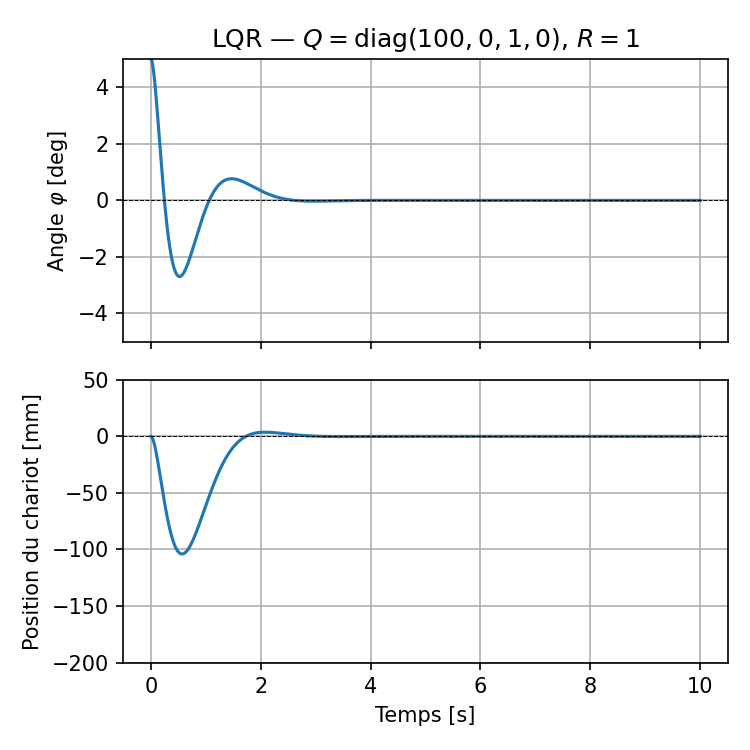
\includegraphics[width=\linewidth]{figures/lqr_x100_xd0_th1_thd0_u1.png}\\[2pt]
    {\scriptsize Pondération forte sur $x$: $q_x = 100$, $q_\varphi = 1$}
  \end{column}
  \begin{column}{0.5\textwidth}
    \centering
    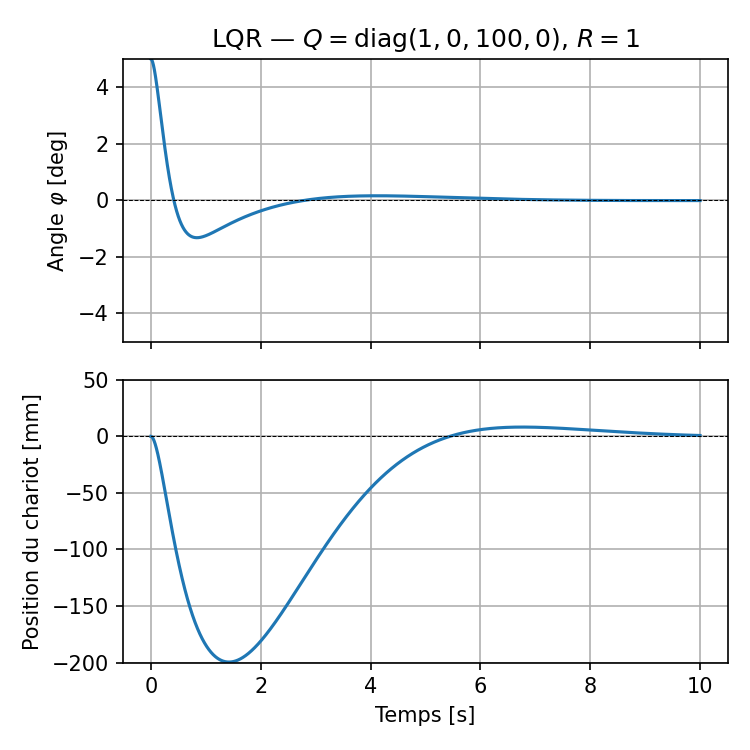
\includegraphics[width=\linewidth]{figures/lqr_x1_xd0_th100_thd0_u1.png}\\[2pt]
    {\scriptsize Pondération forte sur $\varphi$: $q_x = 1$, $q_\varphi = 100$}
  \end{column}
\end{columns}

\end{frame}

%%%%%%%%%%%%%%%%%%%%%%%%%%%%%%%%%%%%%%%%%%%%%%%%

\begin{frame}
\frametitle{Contrôle LQ}
\framesubtitle{Résultats Expérimentaux}

\begin{figure}
    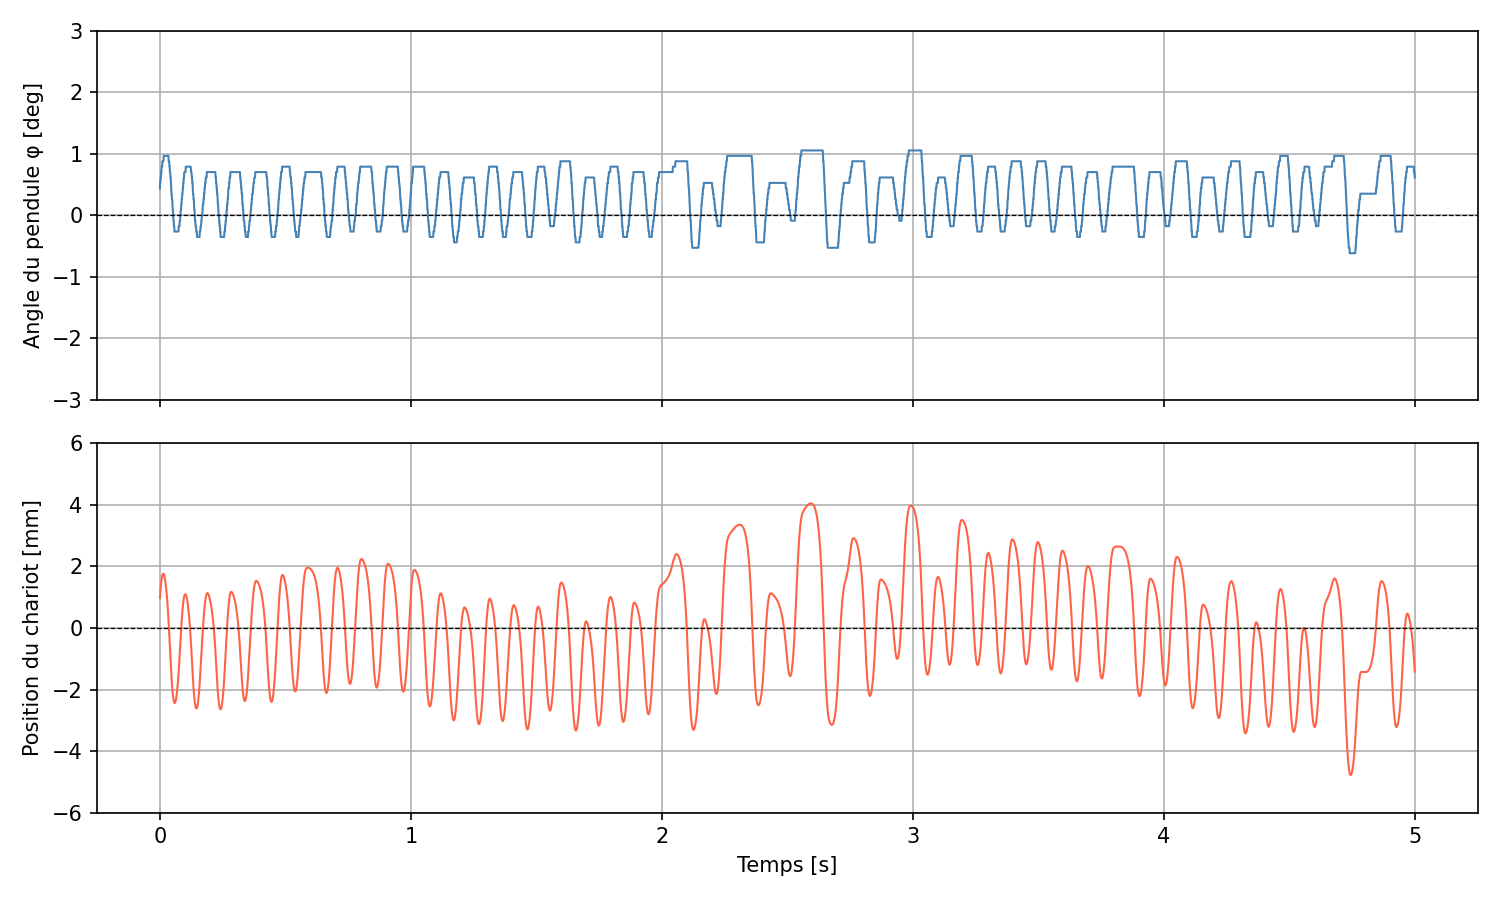
\includegraphics[width=0.9\linewidth]{figures/data_lqr_x1000_xd0_th_1000_thd0_u1_stability.png}\\[2pt]
    
    {\scriptsize $\mathbf{K} = [-31.6\ -23.1\ 92.8\ 18.3]$, stabilité observée de $\pm 1\,\text{deg}$, $\pm 5\,mm$}
\end{figure}

\end{frame}
